\documentclass[11pt]{article}
\title{\bf \underline{High Performance Computing Programming exercises}}
\author{\bf Oliver Tarrant}
\date{}
\usepackage{graphicx}
\usepackage{float}
\textheight=9.1in
\topmargin=-0.7in
\headheight=0pt
\oddsidemargin=-0.25in %length of margin on sides for odd pages
\evensidemargin=-0.25in %length of margin on sides for even pages
\textwidth=6.77in 
\begin{document}
\maketitle
\section{Neutral Theory Simulations}
\subsection*{8)}
\begin{figure}[H]
\begin{center}
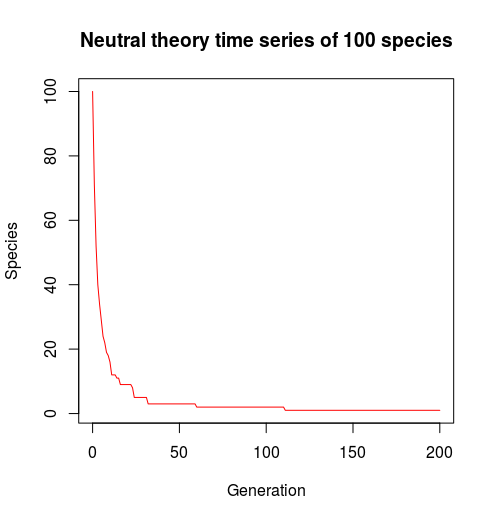
\includegraphics[scale=0.5]{../Results/Plots/Neutral_theory_time_series.png}
\caption{A graph showing the time series of a neutral theory simulation of 100 species over 200 generations with no speciation}
\end{center}
\end{figure}
In this simulation the state will always converge to a singular species if the simualtion is allowed to run for long enough. This is because the simulation loses species whenever the species that dies in the neutral step was the last of it's type. For example, in the first step when there is only one of each species the species which dies is the last of it's type and replaced with one of the other species hence the total species number decreases. However, in this simulation there is no mechanism for a new species to be introduced and hance whilst the species number can go down it can't go up. As there will always be atleast one species, this means that the system will always converge to one species.
\subsection*{12)}
\begin{figure}[H]
\begin{center}
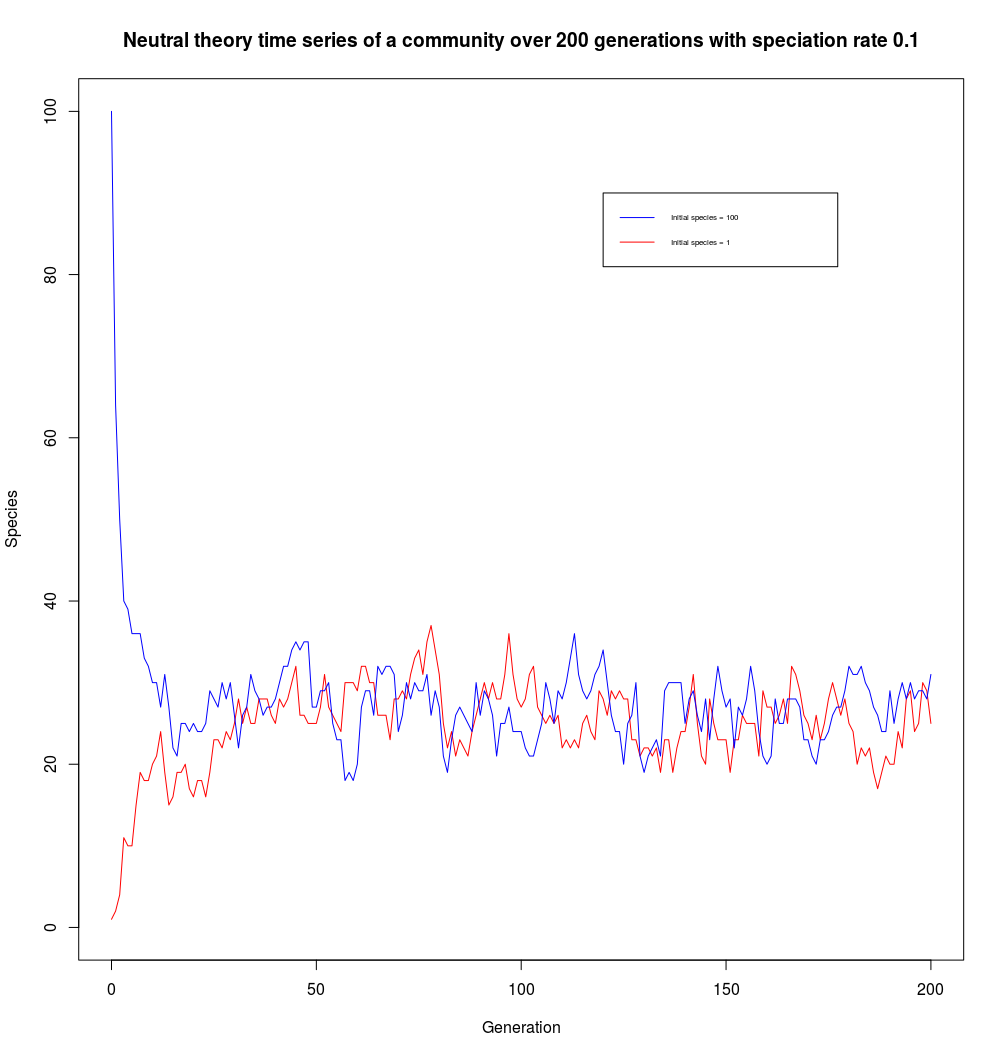
\includegraphics[scale=0.35]{../Results/Plots/Neutral_with_speciation.png} 
\caption{Time series graph of neutral theory simulation with speciation at rate 0.1. The blue line simulates a community which started with 100 unique species and the red line a community that started with just 1 unique species. Both communities had 100 individuals.}
\end{center}
\end{figure}
In this simulation both the community that started with 100 unique species and that with just one species have converge to approximately 30 species after the initial burn in generations. Thus to study the behaviour of a community under this model over time it doesn't matter on the initial state of the community. This is because whilst the number of new species being introduced is happening at a constant rate (in this simulation 0.1) the rate at which species go extinct is dependent on the number of unique species in the community. With the community size constant, the lower the total number of species, the more likely it is that there are more of each species that does exist. The more there is of a species the less likely it is that all of them will die and not be replaced by more of that same species (or other species dieing beign replaced by that species). Thus the lower the number of species the lower the rate at which species go extinct. When the number of species is so that the speciation rate is approximately equal to the extinction rate the behaviour of the time series will level out. This is the behaviour observed as the time series converges to approximately 30 species. When less than this number the speciation rate is higher than the extinction rate and when higher than this number the extinction rate is higher than the speciation rate. 
\subsection*{16)}
\begin{figure}[H]
\begin{center}
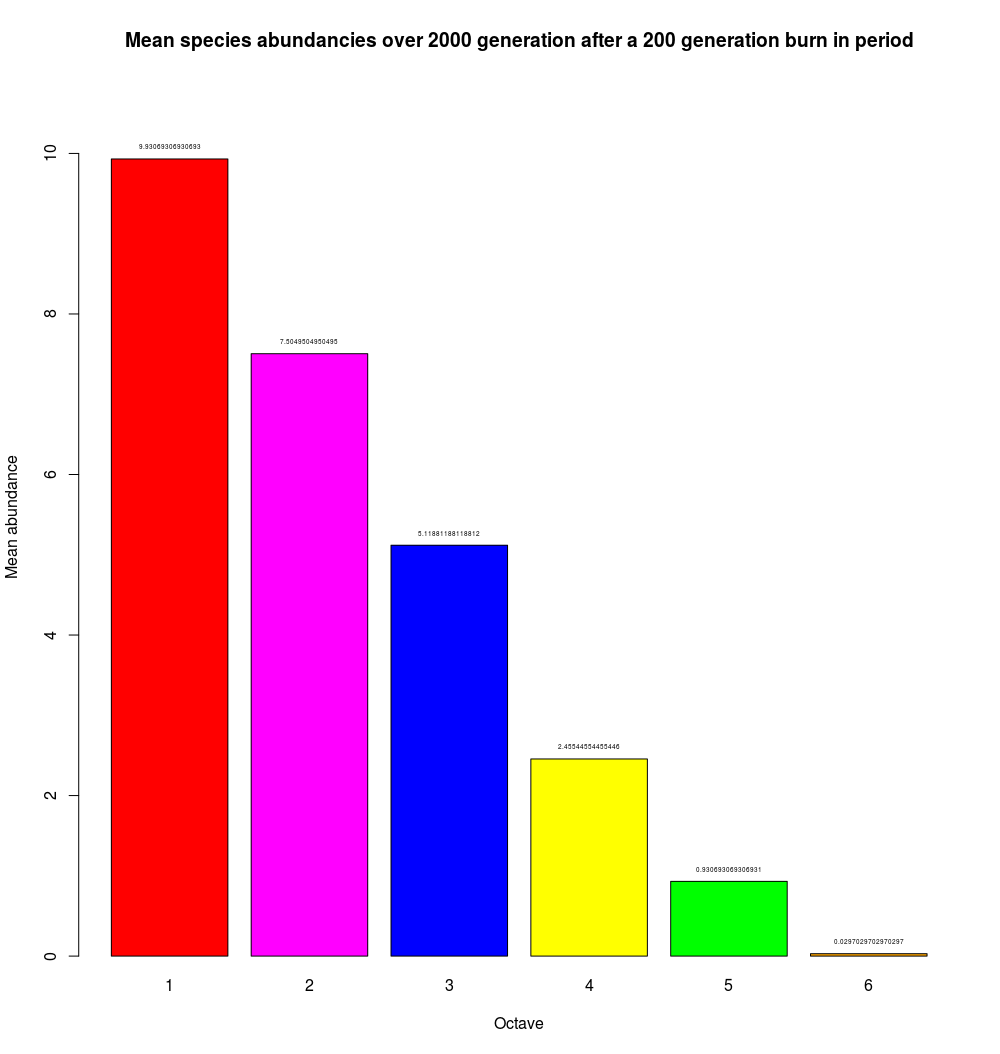
\includegraphics[scale=0.35]{../Results/Plots/Mean_abundancy_octaves.png}
\caption{Bar chart of the average species abundance octave values for a simulation of neutral theory with speciation. The octaves were recorded at every 20 generations for 2000 geneartions starting after an initial burn in period of 200 generations}
\end{center}
\end{figure} 
Once again for this simulation the initial conditions of the community do not matter as by the end fo the burn in period the commnuity characteristics will have stabilised. As explained in question 12 the extinction and speciation rate will be approximately equal and so the number of species will be approximately level. Due to this, although the abundance of particular species will fluctuate, the overall distribution of abundance levels for the community will remain constant. That is because with roughly constant species numbers a decrease in one species will just result in an increase in another one and so overall the effects will balance out across the communtiy. As all communities with converge to the same approximate state no matter what their initial conditions were, for my simulation the initial conditions are irrelivent to the abundancy octaves past the burn in period. 
\subsection*{Challenge A)}
\begin{figure}[H]
\begin{center}
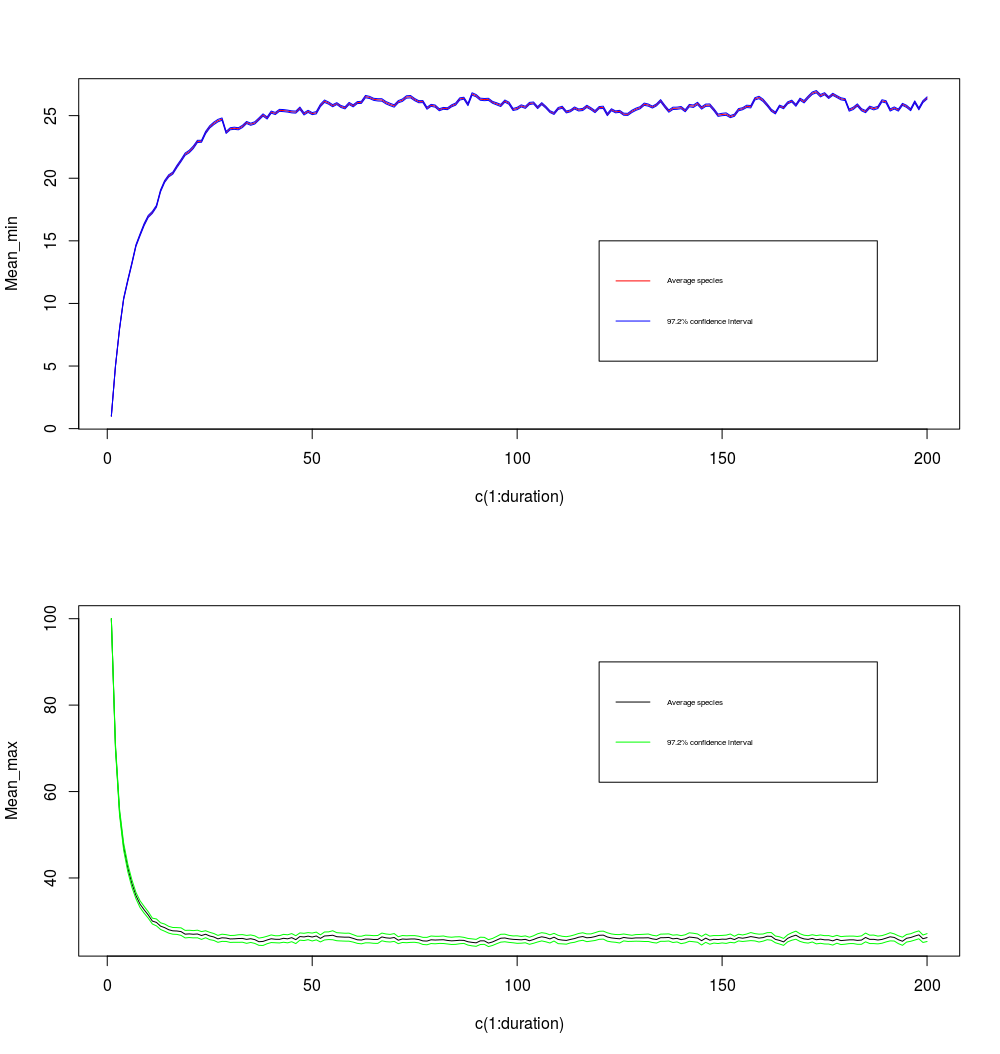
\includegraphics[scale=0.48]{../Results/Plots/challenge_A.png}
\end{center}
\caption{Mean species richness plotted as a function of time both for an initial species richness of 1 and 100. For each graph the plotted value is the average at each time point over 100 simulations with speciation rate 0.1. Dynamic equilibrium is reached when the extinction rate is equal to the speciation rate and judging by the graphs this occurs around 40 generations into the simulations.}
\end{figure}
\subsection*{20)}
\begin{figure}[H]
\begin{center}
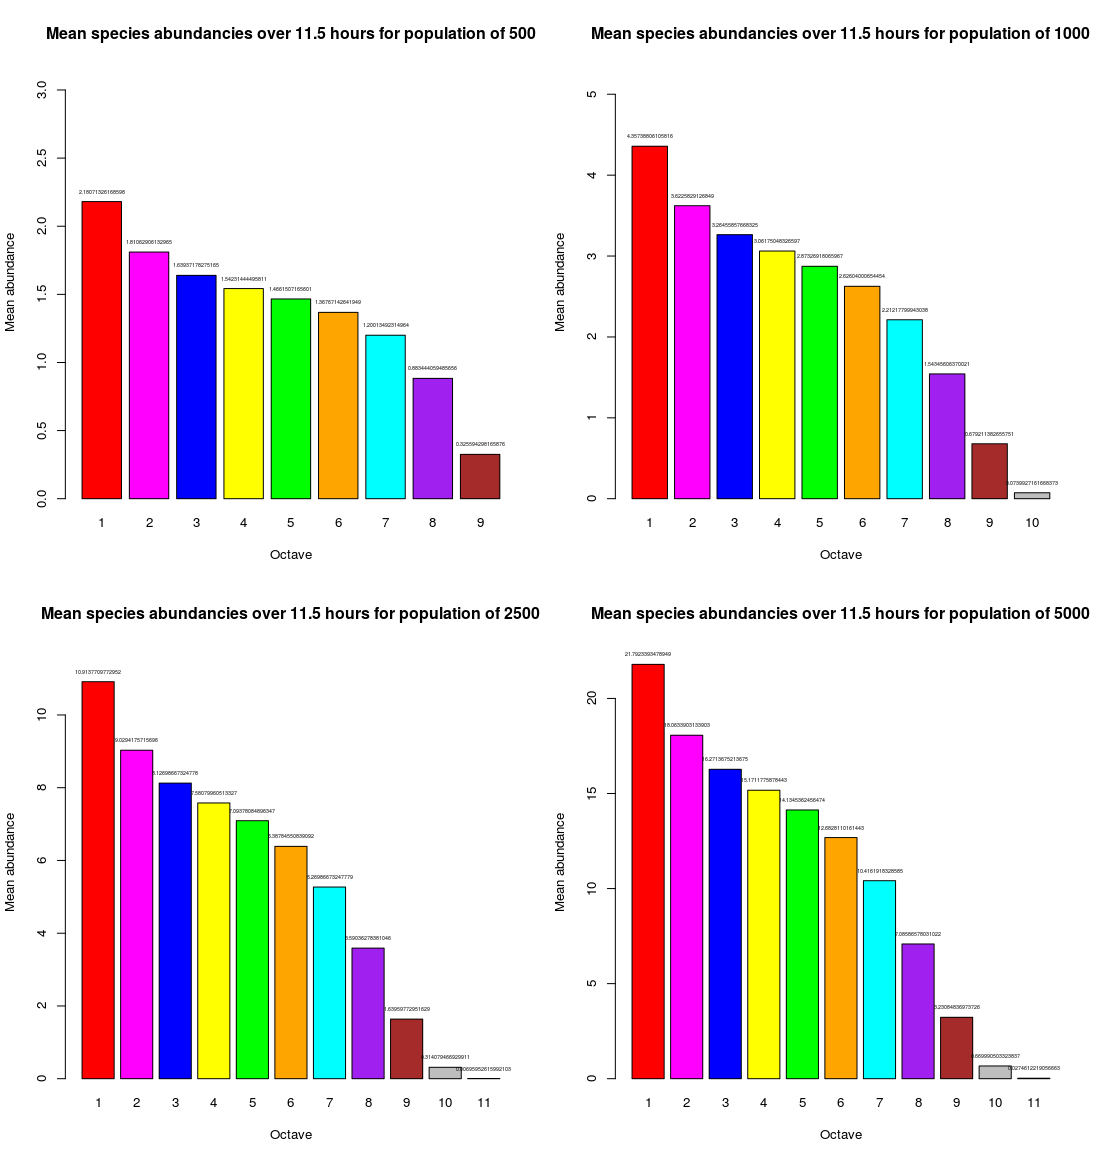
\includegraphics[scale=0.48]{../Results/Plots/Question_20.png}
\caption{Bar charts of the mean species abundance octaves simulated using neutral theory with speciation rate 0.004361 for populations of size 500, 1000, 2500 and 5000. Simulations were run for 11.5 hours and used a burn in period of $8\times Population Size$. The octaves were then recorder every $Population Size \div 10$ generations. 25 simulation runs were performed for each population size and the average was taken for each population size from the entire collection of octaves accumulated across all runs for that population size.}
\end{center}
\end{figure} 
\subsection*{Challenge D)}
Whilst the simulations using HPC took 11.5 hours worth of computing time to complete, the equivilent calculations performed using the coalescence methode took just a few seconds. This is because the calculations in the coalescence methode are performed on only the relevent lineages. Each lineage is traced back until it is a new mutant from an existing lineage. These caluclualtions are performed until only the most recent common ancestor of all the individuals existed and up to this tim point only on the lineages which are ancestors of the end individulas. With each time step you know either two individuals share a common ancestor or that a new species was formed. Either case the number of relevent lineages becomes one less as either two merge or one is removed respectively. Thus once J (community size) steps are perfomed you will be at the most recent common ancestor. At this point the calucualtion is ended. In the HPC calculation every single time step has to be calculated for every individual even those lineages which go extinct. These calculations are performed forwards in time you need to perform every single step to get the final data. 
\subsection*{Fractals in nature - 21)}
For the sierpinski carpet the fractal dimension is $D=log(8)/log(3) = 1.892789...$ and for the Menger sponge $D=log(20)/log(3) = 2.726833...$. These have been calculated using the formula for fractal dimensions $D=log(n)/log(r)$ where n is the number of repeates there is of the shape in one fractal iteration which are found in the next fractal iteration and r is $1/size$ where size is the size of the smaller repeats compared with the previous iteration.\\
The sierpinski carpet is formed by removing the central square from the object in each iteration. In each iteraion, 8 smaller squares are formed, one in each corner and each side of the square removed. Thus n for this fractal is 8. As 3 of these smaller squares now cover the equivilent length or height of the original square these are 1/3 the size ratio of the original square so r = 3.\\
The menger sponge is more difficult. Starting with a cube, at each iteration the cube is broken into 27 cubes arranged in a $3 \times 3 \times 3$ configuration. The middle of which and the middle of each face (6 in total) are removed in the iteration. This is removing 7 of the cubes in the iteration so there are 20 smaller repeates of the original cube remaining thus n = 20. As the 27 smaller cubes create the larger cube and because of the way they are arranged to form it, it is clear that the each has side lengths of 1/3 that of the original cube. Thus the size ratio of these cubes is again 1/3 so r = 3.\\
\subsection*{22)}
\begin{figure}[H]
\begin{center}
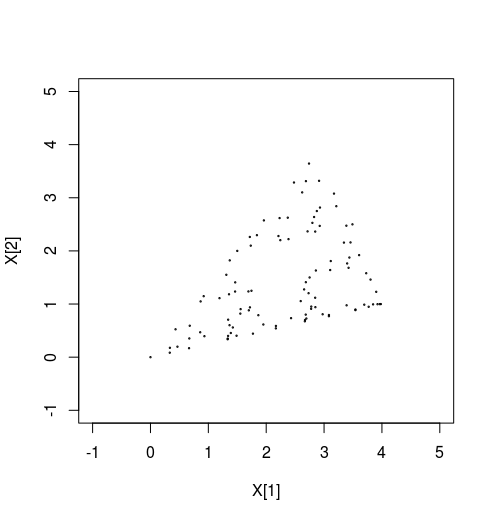
\includegraphics[scale=0.5]{../Results/Plots/Chaos_100.png}
\caption{Chaos game simulated for 100 steps. This is forming the beginings of a Sierpinski Gasket. This is generated because of the pattern of ploting half way between points which creates the fractal effect. }
\end{center}
\end{figure} 
\begin{figure}[H]
\begin{center}
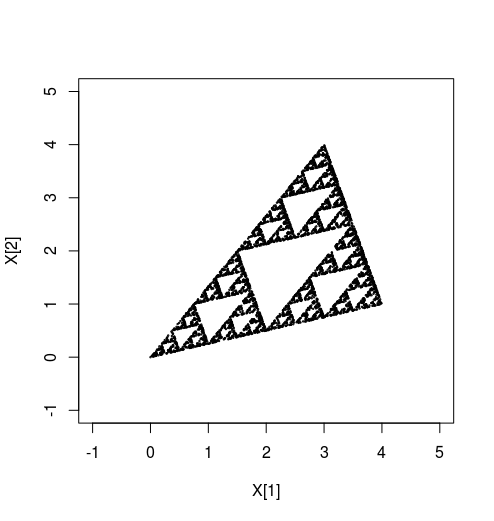
\includegraphics[scale=0.5]{../Results/Plots/Chaos_5000.png}
\caption{Chaos game simulated for 5000 steps. Note how the Sierpinski Gasket is becoming more detailed as the points get more dense and thus the desig more intiricate.}
\end{center}
\end{figure}
\subsection*{Challenge E)}
\begin{figure}[H]
\begin{center}
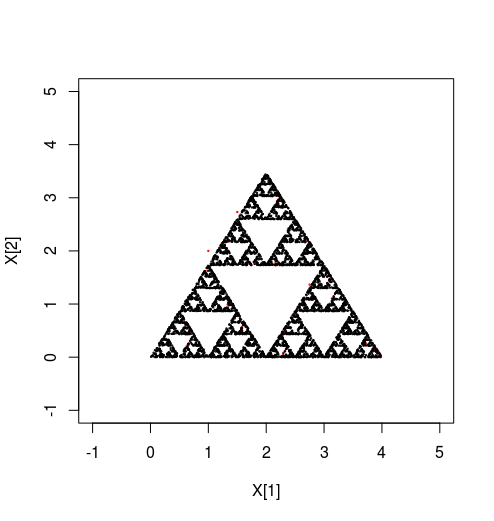
\includegraphics[scale=0.5]{../Results/Plots/Challenge_E.png}
\caption{Chaos game with points positioned as an equiliateral triangle. The initial point doesn't really matter as the algorithm will always converge back to the Sierpinski gasket. For the shown plot my start point was outside of the Sierpinski gasket and the first 100 of the 5000 points are scoloured in red which clearly shows the points quickly converging to the Sierpinski gasket.}
\end{center}
\end{figure}
\subsection*{25)}
The function spiral creates an error as it runs an infinite loop where it calls itself within itself and has no method to end the function and thus the function will run forever so returns an error message.\\
\subsection*{26)}
\begin{figure}[H]
\begin{center}
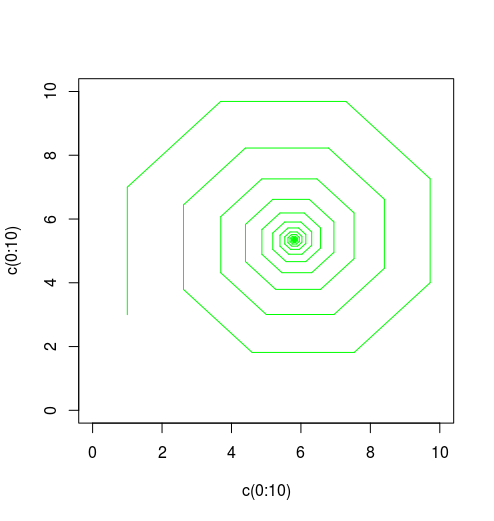
\includegraphics[scale=0.5]{../Results/Plots/Spiral2.png}
\caption{A spiral produced by running spiral2 function starting at (1,3) with initial line legth 4, initial direction $90^{o}$ and minimum line length 0.001. This no longer runs into an error like spiral because the function uses the minimum line length as a cut of point to leave the function when the length of the next line to be drawn in the spiral is less than this length. (Note a blank plot was created first to add the spiral onto.)}
\end{center}
\end{figure}
\subsection*{27}
\begin{figure}[H]
\begin{center}
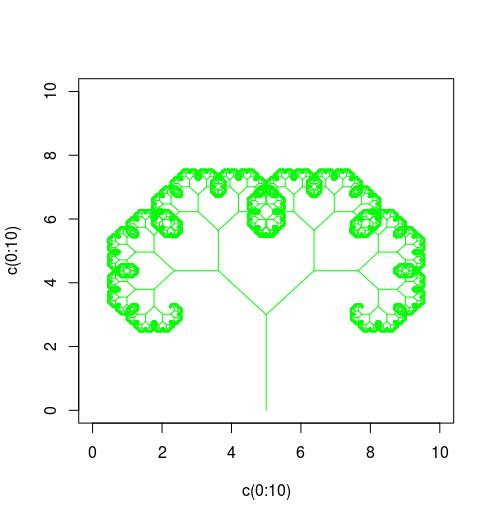
\includegraphics[scale=0.5]{../Results/Plots/Tree.png}
\caption{Animation created usign the tree function. I used an initial start point of (0,5) an initial direction of $90^{o}$, initial line length of 3 and a minimum line length of 0.01. Once again a blank plot was opened first to plot the tree on.}
\end{center}
\end{figure}
\subsection*{29)}
\begin{figure}[H]
\begin{center}
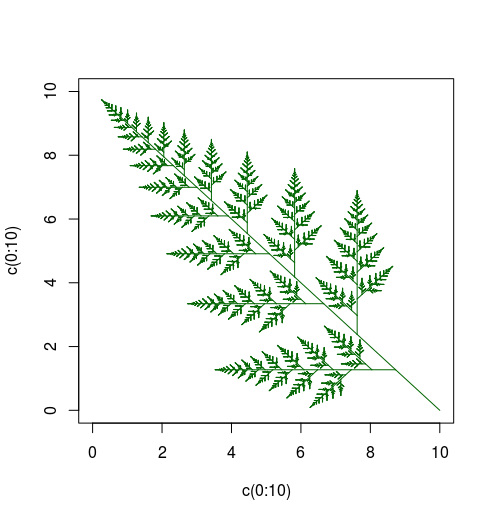
\includegraphics[scale=0.5]{../Results/Plots/Fern.png}
\caption{A fern produced with the function fern2. For this image I used an initial start point of (10,0), an initial direction of $135^{o}$ an initial length of 1.8 a minimum size of 0.01 and an instruction to do the first branch to the left and then alternating from then onwards.}
\end{center}
\end{figure}
\subsection*{Challenge F)}
\begin{figure}[H]
\begin{center}
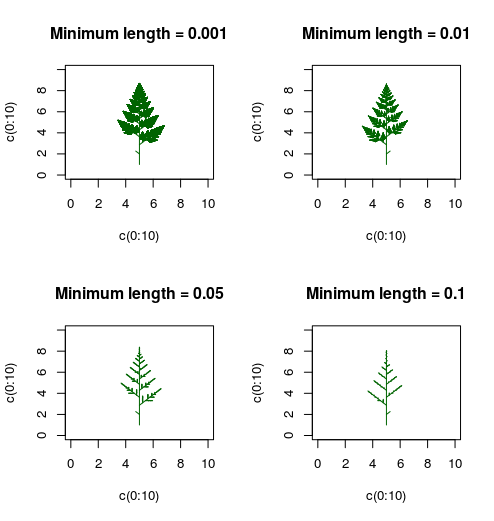
\includegraphics[scale=1]{../Results/Plots/Challenge_F.png}
\caption{Ferns plotted using different values for the minimum line length value before the algorithm terminates. The code I have written also measured how long it took for each length. These times were: 12.101 seconds for a minimum length of 0.001, 0.245 seconds for a minimum length of 0.01, 0.0167 seconds for a minimum length of 0.05 and 0.006 seconds for a minimum length of 0.1. Using these times and the graphs it apperas as if the level of detail and time taken to produce the simulation increase exponentially with respect to the decreased length of the minimum line.  }
\end{center}

\end{figure}
\end{document}